\documentclass[11pt]{article}
\usepackage[utf8]{inputenc}
\usepackage[T1]{fontenc}
\usepackage{amsmath,amssymb,amsthm}
\usepackage{graphicx}
\usepackage{booktabs}
\usepackage{array}
\usepackage[margin=2.4cm]{geometry}
\usepackage{hyperref}
\emergencystretch=2em

% In the repository the figures and the generated numbers live in ../article (written by scripts/permutational.py
% and scripts/symmetry_resolved.py); the arXiv archive (scripts/make_arxiv_btc_sre.sh) copies them next to this file.
\graphicspath{{figures/}{../article/figures/}}
\IfFileExists{generated/permutational.tex}{\input{generated/permutational.tex}}{%
  % generated by scripts/*.py -- do not edit by hand
\newcommand{\PMDevice}{CPU (1 thread)}
\newcommand{\PMMode}{check}
\newcommand{\PMTorch}{2.14.1+cu130}
\newcommand{\PMCuda}{none}
\newcommand{\PMCusolver}{none}
\newcommand{\PMMatmul}{FP32}
\newcommand{\PMOmega}{2}
\newcommand{\PMFullNmax}{8}
\newcommand{\PMFullErr}{6\times10^{-16}}
\newcommand{\PMTrajN}{7}
\newcommand{\PMTrajErr}{3\times10^{-16}}
\newcommand{\PMLibN}{10}
\newcommand{\PMLibErr}{5\times10^{-17}}
\newcommand{\PMLibKrausErr}{7\times10^{-5}}
\newcommand{\PMLibSecGeneric}{0.98}
\newcommand{\PMLibSecBanded}{0.18}
\newcommand{\PMPiqsVersion}{5.3.1}
\newcommand{\PMPiqsGenErr}{7\times10^{-8}}
\newcommand{\PMPiqsNs}{10, 20, 30}
\newcommand{\PMPiqsNmax}{30}
\newcommand{\PMPiqsTrajErr}{3\times10^{-7}}
\newcommand{\PMPiqsBlockErr}{8\times10^{-9}}
\newcommand{\PMPiqsSecOurs}{4.3}
\newcommand{\PMPiqsSecBuild}{0.1}
\newcommand{\PMPiqsSecSolve}{20.0}
\newcommand{\PMPiqsSsNs}{10, 20}
\newcommand{\PMPiqsSsErr}{9\times10^{-9}}
\newcommand{\PMSRRows}{%
10 & 0.266270 & 0.266270 & $3\times10^{-14}$ & 0.924 & 0.910 \\
20 & 0.171321 & 0.171321 & $1\times10^{-16}$ & 1.010 & 0.835 \\
50 & 0.088220 & 0.088220 & $2\times10^{-16}$ & 1.049 & 0.799 \\
100 & 0.051360 & 0.051360 & $1\times10^{-16}$ & 1.055 & 0.789 \\
200 & 0.029244 & 0.029244 & $3\times10^{-16}$ & 1.054 & 0.785 \\
}
\newcommand{\PMSRErr}{3\times10^{-14}}
\newcommand{\PMSRNmax}{200}
\newcommand{\PMProdN}{100}
\newcommand{\PMProdErr}{9\times10^{-14}}
\newcommand{\PMProdPjErr}{2\times10^{-9}}
\newcommand{\PMProdSec}{45}
\newcommand{\PMNs}{10, 20, 30, 40, 50, 60, 80}
\newcommand{\PMNmax}{80}
\newcommand{\PMT}{45}
\newcommand{\PMBatch}{10}
\newcommand{\PMGe}{0.02, 0.05, 0.1, 0.2, 0.5}
\newcommand{\PMGd}{0.005, 0.0125, 0.025, 0.05, 0.125}
\newcommand{\PMConvN}{30}
\newcommand{\PMConvMz}{1\times10^{-6}}
\newcommand{\PMConvTau}{5\times10^{-6}}
\newcommand{\PMFitNmin}{20}
\newcommand{\PMRuleNmin}{30}
\newcommand{\PMSlope}{0.452}
\newcommand{\PMIntercept}{0.98}
\newcommand{\PMTauHeader}{$N$ & $0$ & $0.02$ & $0.05$ & $0.1$ & $0.2$ & $0.5$ & $0.005$ & $0.0125$ & $0.025$ & $0.05$ & $0.125$}
\newcommand{\PMTauRows}{%
10 & 5.49 & 5.19 & 4.76 & 4.20 & 3.46 & 2.62 & 5.39 & 5.26 & 5.10 & 4.73 & 3.88 \\
20 & 9.98 & 8.90 & 7.71 & 6.30 & 4.66 & 3.00 & 9.60 & 9.12 & 8.46 & 7.37 & 5.33 \\
30 & 14.52 & 12.18 & 10.04 & 7.76 & 5.38 & 3.19 & 13.54 & 12.51 & 11.19 & 9.31 & 6.12 \\
40 & 19.06 & 15.05 & 11.88 & 8.79 & 5.86 & 3.31 & 17.16 & 15.46 & 13.46 & 10.74 & 6.65 \\
50 & 23.57 & 17.52 & 13.36 & 9.55 & 6.17 & 3.38 & 20.51 & 18.07 & 15.37 & 11.84 & 6.99 \\
60 & 28.07 & 19.73 & 14.61 & 10.15 & 6.40 & 3.45 & 23.58 & 20.39 & 17.01 & 12.72 & 7.27 \\
80 & 37.08 & 23.51 & 16.54 & 10.99 & 6.72 & 3.52 & 29.08 & 24.41 & 19.68 & 14.05 & 7.63 \\
$\infty$ (MF) & -- & 68.35 & 28.03 & 14.56 & 7.84 & 3.77 & 195.67 & 78.96 & 40.13 & 20.64 & 8.88 \\
}
\newcommand{\PMRuleMin}{-0.067}
\newcommand{\PMRuleMax}{+0.172}
\newcommand{\PMRuleBigMin}{-0.067}
\newcommand{\PMRuleBigMax}{+0.110}
\newcommand{\PMRuleCount}{70}
\newcommand{\PMSecNmax}{690}
\newcommand{\PMSecSweep}{968}
\newcommand{\PMSeconds}{1193}
\newcommand{\PMDimNmax}{91881}
\newcommand{\PMDimFullNmax}{1\times10^{48}}
}
\IfFileExists{generated/symmetry_resolved.tex}{\input{generated/symmetry_resolved.tex}}{%
  % generated by scripts/*.py -- do not edit by hand
\newcommand{\SRDevice}{CPU (2 threads)}
\newcommand{\SRMode}{full}
\newcommand{\SRTorch}{2.14.1+cu130}
\newcommand{\SRCuda}{none}
\newcommand{\SRCusolver}{none}
\newcommand{\SRMatmul}{FP32}
\newcommand{\SRL}{24}
\newcommand{\SRHalf}{12}
\newcommand{\SRQuarter}{6}
\newcommand{\SRDim}{2{,}704{,}156}
\newcommand{\SRNDelta}{8}
\newcommand{\SRChunk}{4}
\newcommand{\SRLanczosM}{40}
\newcommand{\SRDeltas}{-0.75, -0.5, -0.25, 0, 0.25, 0.5, 0.75, 1}
\newcommand{\SRScanL}{8, 10, \dots, 24}
\newcommand{\SRellMinb}{3}
\newcommand{\SRellMinB}{4}
\newcommand{\SRTol}{1\times10^{-12}}
\newcommand{\SRResidual}{3\times10^{-12}}
\newcommand{\SRSecondsGS}{908}
\newcommand{\SRSecondsEnt}{45}
\newcommand{\SRSeconds}{1327}
\newcommand{\SRFFLDense}{14}
\newcommand{\SRFFDenseDev}{2\times10^{-14}}
\newcommand{\SRFFDenseDevS}{1\times10^{-10}}
\newcommand{\SRFFLanczosDev}{2\times10^{-13}}
\newcommand{\SRFFLanczosDevS}{4\times10^{-9}}
\newcommand{\SRFFEDev}{8\times10^{-13}}
\newcommand{\SRPCmp}{1\times10^{-6}}
\newcommand{\SRFullL}{12}
\newcommand{\SRFullDeltas}{-0.5, 0, 0.5, 1}
\newcommand{\SRFullDev}{7\times10^{-13}}
\newcommand{\SRFullOff}{2\times10^{-16}}
\newcommand{\SRRoutesDev}{2\times10^{-16}}
\newcommand{\SRQuSpinL}{20}
\newcommand{\SRQuSpinDelta}{0.5}
\newcommand{\SRQuSpinDev}{5\times10^{-14}}
\newcommand{\SRQuSpinE}{6\times10^{-14}}
\newcommand{\SRInfEll}{3200}
\newcommand{\SRInfGOne}{0.0506605}
\newcommand{\SRInfGRef}{0.0506606}
\newcommand{\SRInfBDev}{2\times10^{-9}}
\newcommand{\SRInfdSEll}{3200}
\newcommand{\SRInfdSRatio}{0.946}
\newcommand{\SRInfdSRatioFirst}{0.881}
\newcommand{\SRInfdSEllFirst}{100}
\newcommand{\SRInfRatio}{3.70}
\newcommand{\SRRingLmax}{3200}
\newcommand{\SRRingGOne}{0.0481}
\newcommand{\SRRingRatio}{3.63}
\newcommand{\SRRingRatioFirst}{2.65}
\newcommand{\SRRingLfirst}{24}
\newcommand{\SRKRows}{%
$-0.75$ & 2.173 & 2.267 & 2.150 & 2.172 & 2.175 & 2.032 \\
$-0.50$ & 1.500 & 1.512 & 1.473 & 1.500 & 1.505 & 1.437 \\
$-0.25$ & 1.192 & 1.189 & 1.178 & 1.210 & 1.217 & 1.167 \\
$+0.00$ & 1.000 & 0.994 & 0.999 & 1.036 & 1.045 & 0.992 \\
$+0.25$ & 0.861 & 0.854 & 0.871 & 0.914 & 0.926 & 0.854 \\
$+0.50$ & 0.750 & 0.744 & 0.769 & 0.819 & 0.833 & 0.737 \\
$+0.75$ & 0.649 & 0.649 & 0.674 & 0.731 & 0.748 & 0.636 \\
$+1.00$ & 0.500 & 0.557 & 0.572 & 0.630 & 0.652 & 0.547 \\
}
\newcommand{\SREqRows}{%
$-0.75$ & 1.439 & 1.247 & 1.259 & 0.727 & 0.8 & 0.0184 & 0.0195 & 0.0184 & 3.60 & 0.0107 \\
$-0.50$ & 1.415 & 1.132 & 1.146 & 0.580 & 1.6 & 0.0262 & 0.0273 & 0.0406 & 3.28 & 0.0261 \\
$-0.25$ & 1.406 & 1.059 & 1.075 & 0.503 & 2.5 & 0.0326 & 0.0337 & 0.0666 & 2.96 & 0.0456 \\
$+0.00$ & 1.405 & 1.004 & 1.019 & 0.452 & 3.6 & 0.0383 & 0.0395 & 0.0969 & 2.65 & 0.0699 \\
$+0.25$ & 1.406 & 0.957 & 0.971 & 0.412 & 4.8 & 0.0434 & 0.0447 & 0.1317 & 2.37 & 0.0998 \\
$+0.50$ & 1.409 & 0.913 & 0.927 & 0.379 & 6.1 & 0.0474 & 0.0491 & 0.1708 & 2.13 & 0.1364 \\
$+0.75$ & 1.413 & 0.869 & 0.880 & 0.349 & 7.7 & 0.0498 & 0.0518 & 0.2128 & 1.94 & 0.1801 \\
$+1.00$ & 1.415 & 0.820 & 0.828 & 0.319 & 9.4 & 0.0494 & 0.0512 & 0.2520 & 1.82 & 0.2300 \\
}
\newcommand{\SRFracHMin}{0.58}
\newcommand{\SRFracHMax}{0.87}
\newcommand{\SRHSampledDevMax}{0.015}
\newcommand{\SRKFourMax}{0.047}
\newcommand{\SRSpreadMax}{9.4}
\newcommand{\SRKFcsDevPct}{0.8}
\newcommand{\SRKFcsMidRange}{-0.5}
\newcommand{\SRKFcsMidRangeHi}{0.75}
\newcommand{\SRKWidthDevPct}{4}
\newcommand{\SRKWidthHalfTwo}{9}
\newcommand{\SRKWidthHalfThree}{11}
\newcommand{\SRSpreadMin}{0.8}
\newcommand{\SRBGrowMin}{6}
\newcommand{\SRHeisKWidthThree}{0.652}
\newcommand{\SRHeisKFcs}{0.557}
\newcommand{\SRRatioMin}{1.82}
\newcommand{\SRRatioMax}{3.60}
\newcommand{\SRdSMin}{0.018}
\newcommand{\SRdSMax}{0.252}
\newcommand{\SRGSlopeRatioMax}{10}
\newcommand{\SRGRelChangeMax}{6}
\newcommand{\SRXXGOne}{0.0395}
\newcommand{\SRXXdS}{0.0969}
\newcommand{\SRCostSectorH}{58}
\newcommand{\SRCostFullH}{2.3}
\newcommand{\SRCostVecRatio}{6.2}
\newcommand{\SRCostRhoRatio}{34}
\newcommand{\SRCostVecGB}{0.022}
}

\DeclareMathOperator{\Tr}{Tr}
\DeclareMathOperator{\Var}{Var}
\newcommand{\C}{\mathbb{C}}
\newcommand{\R}{\mathbb{R}}
\newcommand{\M}{\mathcal{M}}
\newcommand{\D}{\mathcal{D}}
\newcommand{\taumf}{\tau_{\mathrm{MF}}}
\newcommand{\taurule}{\tau_{\mathrm{rule}}}
% code names and paths in typewriter type, breakable at . / _ (url package, loaded by hyperref)
\newcommand{\code}[1]{\nolinkurl{#1}}
\makeatletter\g@addto@macro\UrlBreaks{\do\_}\makeatother

\title{Exact symmetry sectors at work: finite-$N$ lifetimes of a boundary time crystal under local dissipation and
symmetry-resolved entanglement in the XXZ chain}
\author{Irina Nikolaeva \and Andrej Novikov}
\date{}

\begin{document}
\maketitle

\begin{abstract}
When a quantum system has a symmetry, its states and its dynamics live in a block-diagonal algebra, a finite-dimensional
von Neumann algebra of Type~I, whose blocks are much smaller than the Hilbert space. We use this structure, as
implemented in the GPU-capable PyTorch library \texttt{torch\_vn\_algebra}, for two exact finite-size computations.
(A)~For a boundary time crystal of $N$ two-level systems with collective drive and collective decay we add local
emission or local dephasing. These terms do not conserve the total spin, but they commute with the permutations of the
sites. We therefore treat them as completely positive maps between the Schur--Weyl sectors
$\bigoplus_jM_{2j+1}\otimes1_{m_j}$, and evaluate the generator in $O(N^3)$ operations per state, with ten dissipation
rates batched. We compute the lifetime $\tau(N,\gamma)$ of the oscillations for $N\le\PMNmax$ without truncating the
state space. Without local terms the lifetime grows linearly in $N$, in line with the known $1/N$ law of the damping
rate. With local terms it saturates at the mean-field lifetime $\taumf$. We observe that the collective and the local
damping rates approximately add, $1/\tau\approx1/\tau(N,0)+1/\taumf$, with relative deviations of $\tau$ between
$\PMRuleMin$ and $\PMRuleMax$ over all $\PMRuleCount$ data points; this is an observation, not a theorem. (B)~For the ground state of the
XXZ chain with $L=\SRL$ sites, computed for eight anisotropies in one batched Lanczos run, the $U(1)$ sector blocks of
the reduced state give the symmetry-resolved entanglement directly. We determine the widths $B_n$ of the charge
distributions of $\rho_A^n$, test the $1/n$ law of bosonisation, measure the amplitude $G_1(\Delta)$ of the breaking of
equipartition, and obtain the Luttinger parameter from the charge statistics to within $\SRKFcsDevPct\,\%$ for
$\SRKFcsMidRange\le\Delta\le\SRKFcsMidRangeHi$. For free fermions we recover the asymptotic amplitude $1/(2\pi^2)$ of
Bonsignori, Ruggiero and Calabrese and show how slowly it is approached.
\end{abstract}

\noindent\textbf{Keywords:} boundary time crystal; permutational invariance; Schur--Weyl duality; local dissipation;
symmetry-resolved entanglement; XXZ chain; Luttinger parameter; Type~I von Neumann algebra.

\section{Introduction}\label{sec:intro}

Exact numerical results for quantum many-body systems are limited by the dimension of the Hilbert space. A symmetry
reduces this dimension. If a group acts on the Hilbert space $\mathcal H$ and the Hamiltonian, the Lindbladian or the
state commutes with it, the relevant operators lie in the commutant of the group, which in finite dimension is a direct
sum of full matrix algebras with multiplicities,
\begin{equation}\label{eq:typeI}
  \M=\bigoplus_{c=1}^{C}M_{k_c}(\C)\otimes1_{m_c},\qquad \mathcal H=\bigoplus_c\C^{k_c}\otimes\C^{m_c}
\end{equation}
(a finite-dimensional von Neumann algebra of Type~I~\cite{takesaki2002}). A computation that stays in $\M$ only needs
the blocks $A_c\in M_{k_c}$; the multiplicity spaces $\C^{m_c}$ never appear. Superselection rules and conserved charges
lead to the same structure~\cite{bartlett2007}. The idea is old. Here we take it seriously in two places where it gives
data that we have not found in the literature. In both cases the decisive step is to treat an operation that
\emph{changes} the sector, or that \emph{splits} the system, as a map between blocks rather than as an operator on
$\mathcal H$.

\paragraph{(A) Boundary time crystal with local dissipation.} $N$ two-level systems driven and damped collectively form a
boundary time crystal~\cite{iemini2018}: the magnetisation oscillates, and at finite $N$ the oscillations are damped
with a rate that vanishes as $1/N$~\cite{liu2026,nemeth2025}. Real emitters also decay and dephase individually. Such
local terms do not conserve the total spin, and in mean field they turn the limit cycle into a damped
oscillation~\cite{piccitto2021}. How long do the oscillations live at finite $N$ when both mechanisms act? The local
terms are permutation invariant, so the state stays in the Schur--Weyl algebra $\bigoplus_jM_{2j+1}\otimes1_{m_j}$, of
dimension $O(N^3)$ instead of $4^N$. We write the local dissipators as completely positive maps between the sectors $j$
and compute the lifetimes $\tau(N,\gamma)$ for $N\le\PMNmax$ and ten local rates. Permutational invariance with local
dissipation is exploited by several methods and codes~\cite{chase2008,baragiola2010,gegg2017,kirton2017,shammah2018};
what we add are the numbers and an observation about them: the collective and local damping rates combine
approximately additively.

\paragraph{(B) Symmetry-resolved entanglement in the XXZ chain.} For a $U(1)$-symmetric pure state the reduced state
$\rho_A$ of a block $A$ commutes with the charge $Q_A$ of $A$, so it lies in $\bigoplus_qM_{\binom\ell q}$. The blocks
are the symmetry-resolved reduced states~\cite{laflorencie2014,goldstein2018,xavier2018}; their entropies $S(q)$ are
independent of $q$ to leading order (equipartition~\cite{xavier2018}), and the corrections are known exactly for free
fermions~\cite{bonsignori2019}. For the interacting XXZ chain at $L=\SRL$ we obtain the blocks of $\rho_A$ directly
from the sector form of the ground state, for eight anisotropies at once, and use them to measure the widths of the
charge distributions, the breaking of equipartition and the Luttinger parameter.

\paragraph{What is known and what is new.} We state the attribution explicitly, since both topics have a large
literature. \emph{Known:} the linear growth of the lifetime of the boundary time crystal with $N$, i.e.\ the $1/N$
law of its damping rate~\cite{liu2026,nemeth2025}; the damping of the mean-field limit cycle by non-collective
dissipation~\cite{piccitto2021}; the permutational-invariance methods~\cite{chase2008,baragiola2010,gegg2017,kirton2017,
shammah2018}; the identities that relate $S(q)$ to the charge distributions and the free-fermion asymptotics
$G_1\to1/(2\pi^2)$ of the equipartition breaking~\cite{bonsignori2019}; the bosonisation background and the
relation between charge fluctuations and the Luttinger parameter~\cite{goldstein2018,song2012,estienne2021}.
\emph{New, as far as we know:} the finite-$N$ lifetimes $\tau(N,\gamma)$ with local emission or dephasing for
$N\le\PMNmax$, computed exactly in the Schur--Weyl decomposition; the observed approximate additivity of the collective
and local damping rates, with the structure of its deviations; the widths $B_n$ of the charge distributions of
$\rho_A^n$ and a test of the $1/n$ law at $L=\SRL$; the amplitudes $G_1(\Delta)$ across anisotropies; and a
determination of the Luttinger parameter from the charge statistics, to within $\SRKFcsDevPct\,\%$ for
$\SRKFcsMidRange\le\Delta\le\SRKFcsMidRangeHi$. The computations use the library
\texttt{torch\_vn\_algebra}~\cite{lib}, built on PyTorch~\cite{paszke2019}; brief accounts of both computations appear
as use cases in its description~\cite{lib}. All numbers below come from CPU runs of the scripts in its repository.

\paragraph{Organisation.} Section~\ref{sec:method} describes the block-diagonal representation, the Schur--Weyl
decomposition with local dissipators as maps between sectors, and the $U(1)$ sectors of a bipartition.
Section~\ref{sec:btc} treats the boundary time crystal, Section~\ref{sec:sre} the symmetry-resolved entanglement.
Section~\ref{sec:validation} lists the checks, and Section~\ref{sec:outlook} gives an outlook.

\section{Method: computing in the blocks}\label{sec:method}

\subsection{Block-diagonal algebras, states and maps between sectors}\label{sec:typeI}

Let $\M$ be as in~\eqref{eq:typeI}. An element of $\M$ is a list of blocks $A=\bigoplus_cA_c$, and the trace of
$\mathcal H$ restricts to $\Tr_{\mathcal H}(A\otimes1)=\sum_cm_c\Tr A_c$. A state $\rho$ on $\mathcal H$ that commutes
with the symmetry has the form $\rho=\bigoplus_c\sigma_c\otimes1_{m_c}/m_c$, and we store the blocks $\sigma_c$, which
satisfy $\sum_c\Tr\sigma_c=1$ and $\Tr_{\mathcal H}(\rho A)=\sum_c\Tr(\sigma_cA_c)$. In the language of~\cite{lib},
$\sigma$ is the density of the state with respect to the ``blunt'' trace $\sum_c\Tr A_c$; $p_c=\Tr\sigma_c$ is the
probability of the sector $c$.

Every normal completely positive map $\Phi:\M\to\M$ is a sum of maps between blocks,
\begin{equation}\label{eq:intersector}
  \Phi(\sigma)_d=\sum_c\sum_iK^{dc}_i\,\sigma_c\,K^{dc*}_i,\qquad K^{dc}_i:\C^{k_c}\to\C^{k_d}.
\end{equation}
This is the form in which a symmetric dissipator enters. A Lindblad term $\sum_i\D[L_i]$, $\D[L]\rho=L\rho L^*-\frac12\{L^*L,\rho\}$, whose individual
jump operators $L_i$ do not commute with the symmetry but whose sum does, need not be of the form $\D[L]$ with $L\in\M$.
It is, however, of the form $\Phi(\rho)-\frac12\{\Phi^*(1),\rho\}$ with the completely positive map
$\Phi(\rho)=\sum_iL_i\rho L_i^*$, which maps $\M$ into $\M$, and with $\Phi^*(1)=\sum_iL_i^*L_i\in\M$. The generator
therefore acts on the blocks: a Hamiltonian and jump operators in $\M$ act inside the blocks, and a map~\eqref{eq:intersector}
couples them. In the library this is the class \code{InterSectorChannel}, which \code{dynamics.lindblad_evolve} accepts
as a jump~\cite{lib}.

\subsection{Schur--Weyl sectors of \texorpdfstring{$N$}{N} two-level systems}\label{sec:schurweyl}

By Schur--Weyl duality~\cite{fulton1991}, the symmetric group permuting the factors of $(\C^2)^{\otimes N}$ and the
collective $SU(2)$ generate each other's commutants,
\begin{equation}\label{eq:sw}
  (\C^2)^{\otimes N}=\bigoplus_jV_j\otimes\C^{m_j},\qquad \dim V_j=2j+1,\quad
  m_j=\binom N{N/2-j}-\binom N{N/2-j-1},
\end{equation}
$j=N/2,N/2-1,\dots\ge0$. The permutation-invariant operators form $\M=\bigoplus_jM_{2j+1}(\C)\otimes1_{m_j}$. A state
of this algebra has $\sum_j(2j+1)^2=O(N^3)$ entries, for $N=\PMNmax$ exactly $\PMDimNmax$, whereas a density matrix on
$(\C^2)^{\otimes\PMNmax}$ has $4^{\PMNmax}\approx\PMDimFullNmax$ entries. The blocks $\sigma_j$ are the
``Dicke-basis'' densities of PIQS~\cite{shammah2018}. The collective operators $J_a=\frac12\sum_i\sigma_a^{(i)}$ act in
block $j$ as the spin-$j$ matrices in the basis $|j,m\rangle$.

\paragraph{Local dissipators as maps between sectors.} For a single-site operator $L\in\{\sigma_-,\sigma_+,\sigma_z\}$
the map $\Phi(X)=\sum_{i=1}^NL^{(i)}XL^{(i)*}$ commutes with the permutations. To find its Kraus operators on the blocks
we restrict to the last site and branch $N\to N-1$: the multiplicity space $\C^{m_j}$ is the direct sum of the
multiplicity spaces of $j_1=j\pm\frac12$ for $N-1$ sites, $L^{(N)}$ preserves $j_1$, and all $N$ sites contribute
equally. This gives
\begin{equation}\label{eq:kraus}
  \Phi(\sigma)_{j'}=\sum_j\sum_{j_1}K^{j'j}_{j_1}\,\sigma_j\,K^{j'j*}_{j_1},\qquad
  K^{j'j}_{j_1}=\Bigl(\frac{N\,m^{(N-1)}_{j_1}}{m^{(N)}_j}\Bigr)^{1/2}
  \bigl\langle j_1,\tfrac12;j'\bigr|\,1\otimes L\,\bigl|j_1,\tfrac12;j\bigr\rangle ,
\end{equation}
with $|j'-j|\le1$, $j_1\in\{j\pm\frac12\}\cap\{j'\pm\frac12\}$, and the coupled multiplets of $V_{j_1}\otimes\C^2$
(Clebsch--Gordan coefficients of $j_1\otimes\frac12$) in the last factor. Each $K$ has a single non-zero diagonal, and
$\Phi^*(1)=\sum_iL^{(i)*}L^{(i)}$ equals $N/2+J_z$, $N/2-J_z$ or $N$ for $\sigma_-$, $\sigma_+$, $\sigma_z$. Closed
forms of these coefficients are given in~\cite{chase2008,baragiola2010,shammah2018}; we verify ours against the exact
generator on $(\C^2)^{\otimes N}$ and against PIQS (Section~\ref{sec:validation}). The same symmetry is used by
PsiQuaSP~\cite{gegg2017} and by Kirton and Keeling~\cite{kirton2017}.

\paragraph{Banded evaluation and batching.} In the library, \code{PermutationalSystem(N)} is the algebra with these
sectors, and \code{local_jump} returns $\Phi$ as an \code{InterSectorChannel} of Kraus rank two. With it the generic
integrator handles collective jumps as operators and local ones as maps between sectors. Its dense Kraus tensor has
$2C^2k_{\max}^2$ entries ($C=\lfloor N/2\rfloor+1$ sectors, $k_{\max}=N+1$), which limits this route to a few tens of
spins. Every operator in the generators below is banded in the basis $|j,m\rangle$: $J_\pm$ and $\sigma_\pm$ shift $m$
by one, and the local maps change $j$ by at most one. \code{PermutationalLindbladian} therefore evaluates
\begin{multline}\label{eq:general}
  \dot\sigma=-i[\omega_xJ_x+\omega_yJ_y+\omega_zJ_z,\sigma]+\Gamma_-\D[J_-]\sigma+\Gamma_+\D[J_+]\sigma
  +\Gamma_z\D[J_z]\sigma\\
  +\gamma_-\sum_i\D[\sigma_-^{(i)}]\sigma+\gamma_+\sum_i\D[\sigma_+^{(i)}]\sigma+\gamma_z\sum_i\D[\sigma_z^{(i)}]\sigma
\end{multline}
as a sum of shifted elementwise products of the blocks and a tridiagonal Hamiltonian part. This costs
$O(N^3)$ operations per state instead of $O(N^4)$ for dense block products, and every coefficient may be a vector, one
entry per batch element. With $\omega_x=\omega_z=0$ every term maps real matrices to real matrices, and the
computation runs in the real algebra $\bigoplus_jM_{2j+1}(\R)$. Finally, \code{PermutationalSystem(N, j_min)} keeps
only the sectors $j\ge j_{\min}$. This compression generates a trace-decreasing completely positive semigroup whose
error on an observable $A$ is bounded by $2\|A\|$ times the lost weight. We use it only where it is exact: without
local terms only the sector $j=N/2$ is populated.

\subsection{\texorpdfstring{$U(1)$}{U(1)} sectors of a bipartition}\label{sec:u1}

A spin-$\frac12$ chain of $L$ sites with a Hamiltonian that conserves $S^z_{\rm tot}$ is block diagonal in the number
$N$ of up spins: $\M_L=\bigoplus_{N=0}^LM_{\binom LN}(\C)$. Its ground state at $S^z_{\rm tot}=0$ is a vector in the
sector $N=L/2$, of dimension $\binom{L}{L/2}$ ($\SRDim$ for $L=\SRL$). For a block $A=\{0,\dots,\ell-1\}$ and its
complement $B$, the sector $N$ splits as
\begin{equation}\label{eq:fused}
  \C^{\binom LN}=\bigoplus_{q}\C^{\binom\ell q}\otimes\C^{\binom{L-\ell}{N-q}},
\end{equation}
the sector $N$ of the fused tensor product $\M_A\otimes_f\M_B$ of the two chain algebras, in which only the total
charge is conserved (\code{composite.fused_tensor_product} in~\cite{lib}). In this layout $|\psi\rangle$ is a list of
matrices $\Psi_q\in\C^{\binom\ell q\times\binom{L-\ell}{N-q}}$, and
\begin{equation}\label{eq:rhoA}
  \rho_A=\Tr_B|\psi\rangle\langle\psi|=\bigoplus_{q=0}^{\ell}\Psi_q\Psi_q^*\ \in\ \M_A=\bigoplus_qM_{\binom\ell q}(\C).
\end{equation}
The matrix $|\psi\rangle\langle\psi|$, of dimension $\binom{24}{12}^2\approx7.3\times10^{12}$ at $L=24$, is never formed.
The minimal central projections of $\M_A$ are the spectral projections $\Pi_q$ of $Q_A$, so the sector probabilities
$p(q)=\Tr\Psi_q\Psi_q^*$ and the spectra of the normalised blocks are exactly the symmetry-resolved data.

For the XXZ chain the anisotropy $\Delta$ multiplies only the diagonal $S^zS^z$ part of the sector Hamiltonian. The
Hamiltonians for several $\Delta$ therefore form one batched sparse operator with a shared hopping part
(\code{krylov.SparseSectorHamiltonian}), and one batched Lanczos run gives all ground states.

\section{Part A: a boundary time crystal under local dissipation}\label{sec:btc}

\subsection{Model and observables}\label{sec:btc-model}

We consider
\begin{equation}\label{eq:btc}
  \dot\rho=-i[\omega J_x,\rho]+\frac{\kappa}{S}\,\D[J_-]\rho
  +\gamma\sum_{i=1}^N\D[\sigma_-^{(i)}]\rho+\gamma_\phi\sum_{i=1}^N\D[\sigma_z^{(i)}]\rho,\qquad S=\frac N2 .
\end{equation}
For $\gamma=\gamma_\phi=0$ this is the boundary time crystal of Iemini et al.~\cite{iemini2018}. For $\omega>\kappa$ the
magnetisation $m_z=\langle J_z\rangle/S$ oscillates, and at finite $N$ the oscillations are damped with a rate that
vanishes as $1/N$; for $\omega\gg\kappa$ the rate is $3\kappa/(2N)$ for oscillations from all spins
down~\cite{liu2026,nemeth2025}. The mean-field equations become exact as $N\to\infty$ at fixed times; Carollo and Lesanovsky~\cite{carollo2021}
prove this for open Dicke models and note that the proof adapts to all-to-all spin models and to individual spin
dissipation. In mean field, non-collective dissipation damps the limit cycle~\cite{piccitto2021}.
Robustness of boundary time crystals has also been studied in multi-level settings~\cite{prazeres2021}, and
single-particle dephasing in a related synchronised phase~\cite{tucker2018}.

We take $\omega=\PMOmega\kappa$ and all spins down at $t=0$. In the computation we drive about $y$ instead of $x$. The
rotation $e^{-i\pi J_z/2}$ maps one drive to the other and commutes with every dissipator in~\eqref{eq:btc}, so $m_z(t)$
is unchanged, and the generator becomes real (Section~\ref{sec:schurweyl}).

\paragraph{Lifetime.} Let $t_0=0<t_1<t_2<\dots$ be the extrema of $m_z(t)$ and $a_k=|m_z(t_{k+1})-m_z(t_k)|/2$ the
half-swings. The lifetime $\tau$ is the first time at which $a_k$ falls below $a_0/e$, with log-linear interpolation
between the midpoints $(t_k+t_{k+1})/2$ of consecutive swings. A run that ends before this happens is censored.

\paragraph{Mean-field limit.} For $N\to\infty$, $m=\langle\mathbf J\rangle/S$ obeys (drive about $y$)
\begin{equation}\label{eq:mf}
  \dot m_x=\omega m_z+\kappa m_xm_z-\Gamma_2m_x,\quad \dot m_y=\kappa m_ym_z-\Gamma_2m_y,\quad
  \dot m_z=-\omega m_x-\kappa(m_x^2+m_y^2)-\gamma(1+m_z),
\end{equation}
with $\Gamma_2=\gamma/2+2\gamma_\phi$. Without local terms the orbit from $m=(0,0,-1)$ is closed and $m_z$ does not decay.
We define $\taumf(\gamma)$ and $\taumf(\gamma_\phi)$ as the lifetimes of the solutions of~\eqref{eq:mf}, integrated
to $\kappa t=600$.

\paragraph{Protocol.} For every $N\in\{\PMNs\}$ one batched run holds the $\PMBatch$ parameter sets
$\gamma/\kappa\in\{\PMGe\}$ (with $\gamma_\phi=0$) and $\gamma_\phi/\kappa\in\{\PMGd\}$ (with $\gamma=0$). The two
lists are paired so that $\gamma=4\gamma_\phi$, i.e.\ equal transverse rates $\Gamma_2$. The generator is integrated with
the classical fourth-order Runge--Kutta method (RK4) in the real algebra $\bigoplus_jM_{2j+1}(\R)$, with all $N/2+1$ (or
$(N+1)/2$) sectors kept. The step is $h\le3.5/r$, with $r$ an upper bound on the spectral radius of the generator, and
$m_z$ is sampled every $\kappa\,\delta t=0.05$. A batch element is dropped once its lifetime is settled
($t>\tau+6/\kappa$), and the run ends at $\kappa t=\PMT$. The runs without local terms use the single block $M_{N+1}$
($j_{\min}=N/2$) and last until $\kappa t=0.6N+15$.

\subsection{Results}\label{sec:btc-results}

\begin{table}[t]
\centering\small
\caption{Lifetime $\kappa\tau$ of the oscillations of $m_z$ in~\eqref{eq:btc}, $\omega=\PMOmega\kappa$, from all spins
down: without local terms (column~$0$), with local emission $\gamma/\kappa$ and with local dephasing $\gamma_\phi/\kappa$.
Columns at equal position in the two groups have equal $\Gamma_2=\gamma/2+2\gamma_\phi$. Last row: mean field
($N\to\infty$), Eq.~\eqref{eq:mf}. No entry is censored.}\label{tab:btc}
\begin{tabular}{r|c|ccccc|ccccc}
\toprule
 & & \multicolumn{5}{c|}{local emission $\gamma/\kappa$} & \multicolumn{5}{c}{local dephasing $\gamma_\phi/\kappa$}\\
\PMTauHeader\\
\midrule
\PMTauRows
\bottomrule
\end{tabular}
\end{table}

\begin{figure}[t]
\centering
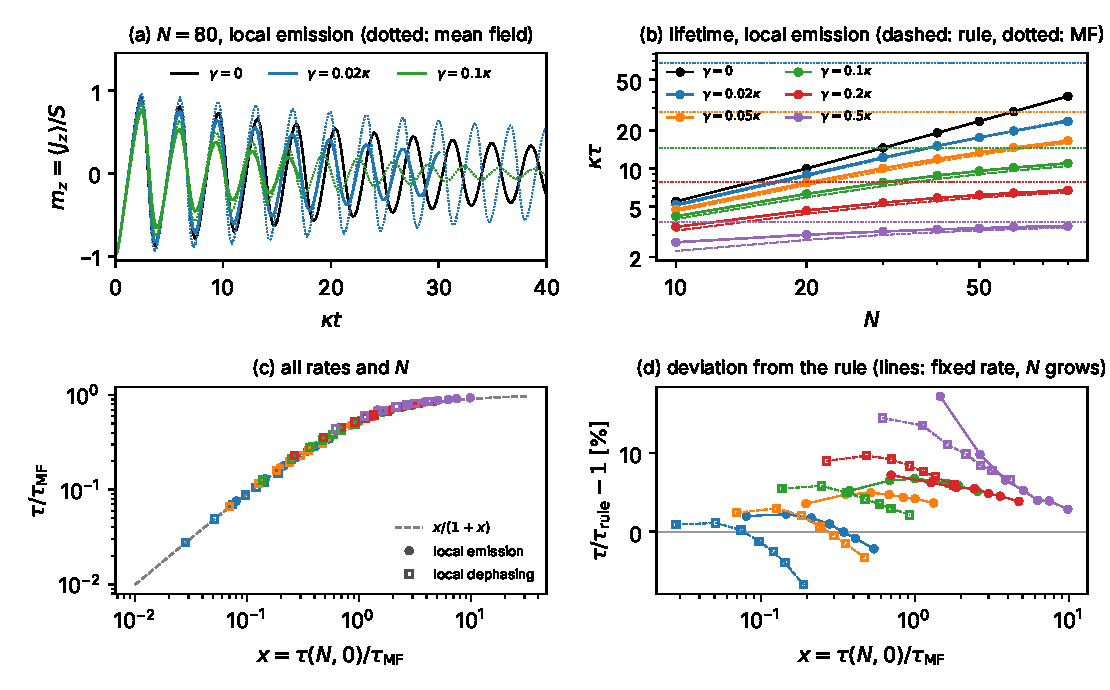
\includegraphics[width=\textwidth]{permutational.pdf}
\caption{(a) $m_z(t)$ for $N=\PMNmax$ without and with local emission ($\gamma=0.02\kappa$, $0.1\kappa$), and the
mean-field curves (dotted). (b) $\tau(N,\gamma)$ for local emission; dotted: $\taumf(\gamma)$, dashed: the additive
rule~\eqref{eq:rule}. (c) All lifetimes with a finite mean-field limit, $\tau/\taumf$ against
$x=\tau(N,0)/\taumf$; the dashed curve $x/(1+x)$ is~\eqref{eq:rule}. (d) The relative deviation from the rule; points
of equal rate are joined, $N$ increasing to the right (filled: emission, open: dephasing).}\label{fig:btc}
\end{figure}

Table~\ref{tab:btc} and Figure~\ref{fig:btc} summarise the sweep; the largest run, $N=\PMNmax$ with $\PMBatch$ parameter
sets, took $\PMSecNmax$~s on one CPU thread.

\paragraph{Without local terms} the lifetime grows linearly. A least-squares fit for $\PMFitNmin\le N\le\PMNmax$ gives
\begin{equation}\label{eq:linear}
  \kappa\tau(N,0)\approx\PMSlope\,N+\PMIntercept .
\end{equation}
The linear growth is the known $1/N$ law of the damping rate~\cite{liu2026,nemeth2025}. In the perturbative regime
$\omega\gg\kappa$ the rate $3\kappa/(2N)$ of~\cite{liu2026,nemeth2025} corresponds to $\kappa\tau\approx2N/3$. Our
$\omega=\PMOmega\kappa$ lies outside that regime, and the slope $\PMSlope$ is smaller. Only this value of the slope at
$\omega=\PMOmega\kappa$ is new.

\paragraph{With local terms} the lifetime saturates at the mean-field value as $N$ grows (last row of
Table~\ref{tab:btc}). For example, with $\gamma=0.5\kappa$ the lifetime grows only from $2.62$ to $3.52$ between $N=10$
and $N=\PMNmax$, against $\kappa\taumf=3.77$. Local emission damps more strongly than local dephasing at equal
transverse rate $\Gamma_2$ (compare $\gamma=0.1\kappa$, $\kappa\taumf=14.56$, with $\gamma_\phi=0.025\kappa$,
$\kappa\taumf=40.13$). In~\eqref{eq:mf}, emission also relaxes $m_z$ directly through the term $-\gamma(1+m_z)$.

\subsection{Approximate additivity of the damping rates}\label{sec:btc-rule}

The collective damping vanishes as $N\to\infty$; the local damping does not. We find that the two combine
approximately like independent decay rates,
\begin{equation}\label{eq:rule}
  \frac1{\tau(N,\gamma)}\approx\frac1{\taurule}=\frac1{\tau(N,0)}+\frac1{\taumf(\gamma)} ,
\end{equation}
for local emission and local dephasing alike. In the variables $x=\tau(N,0)/\taumf$ and $\tau/\taumf$,
\eqref{eq:rule} is the single curve $x/(1+x)$. All data lie close to it (Figure~\ref{fig:btc}c), although $x$ spans
more than two decades. The crossover at which the local damping takes over, $x=1$, lies at
$N^*\approx\kappa\taumf/\PMSlope$ by~\eqref{eq:linear}. For instance, for $\gamma=0.1\kappa$ we have $\kappa\tau(30,0)=14.52$
against $\kappa\taumf=14.56$. The rule then predicts $\kappa\tau=7.27$ at $N=30$, and we find $7.76$.

\paragraph{Size and structure of the deviations.} Over the $\PMRuleCount$ entries of Table~\ref{tab:btc} with finite
$\tau$ and $\taumf$, $\tau/\taurule-1$ lies between $\PMRuleMin$ and $\PMRuleMax$, and between $\PMRuleBigMin$ and
$\PMRuleBigMax$ for $N\ge\PMRuleNmin$. The deviation has a structure (Figure~\ref{fig:btc}d):
\begin{itemize}\itemsep0pt
\item for the larger rates $\tau$ exceeds $\taurule$, by an amount that decreases at large $N$ (for $\gamma=0.5\kappa$
from $+17\,\%$ at $N=10$ to $+3\,\%$ at $N=\PMNmax$);
\item for the smallest rates the deviation decreases through zero as $N$ grows, so that $\tau<\taurule$ at the largest
$N$ (for $\gamma_\phi=0.005\kappa$ it reaches $\PMRuleBigMin$ at $N=\PMNmax$);
\item at equal $x$, local dephasing deviates more than local emission.
\end{itemize}
A heuristic reading of~\eqref{eq:rule} is that the envelope of the oscillation is the product of a collective and a
local decay factor; if both were exponential, their rates would add, up to the offset by the midpoint of the first
swing that our definition of $\tau$ contains. The deviations indicate that the decay is not simply a product of two
independent exponentials. We therefore
state~\eqref{eq:rule} as an \emph{observation} for this model, these rates, $\omega=\PMOmega\kappa$ and this
definition of the lifetime, valid to within the range just given. We have no proof of it, and our data do not
establish it as an asymptotic law for $N\to\infty$ at fixed rate. The trend of the smallest rates suggests that the
deviations at larger $N$ need not stay inside the range found here.

\subsection{Relation to known results}\label{sec:btc-known}

Without local terms, the growth of the lifetime with $N$ is the known $1/N$ law of the damping
rate~\cite{liu2026,nemeth2025}; our contribution here is only the slope~\eqref{eq:linear} at $\omega=\PMOmega\kappa$.
The damping of the mean-field limit cycle by non-collective dissipation is due to Piccitto et
al.~\cite{piccitto2021}; for local terms it follows directly from~\eqref{eq:mf}, which is how we compute $\taumf$.
That local dephasing and local losses wash out the oscillations at finite $N$ was shown with PIQS for
$N=30$~\cite{shammah2018}. New, as far as we know, are the finite-$N$ lifetimes with local emission or dephasing for
$N$ up to $\PMNmax$ in Table~\ref{tab:btc}, the approximate additivity~\eqref{eq:rule} and the structure of its
deviations. The superradiance checks of Section~\ref{sec:validation} reproduce textbook results~\cite{dicke1954,gross1982}.

\section{Part B: symmetry-resolved entanglement in the XXZ chain}\label{sec:sre}

\subsection{Model and resolved quantities}\label{sec:sre-model}

We consider
\begin{equation}\label{eq:xxz}
  H=\sum_{\langle ij\rangle}\bigl(S^x_iS^x_j+S^y_iS^y_j+\Delta S^z_iS^z_j\bigr),\qquad -1<\Delta\le1,
\end{equation}
on $L=\SRL$ sites with periodic or open boundary conditions, and its ground state in the sector $S^z_{\rm tot}=0$. The
low-energy theory is a Luttinger liquid with the Bethe-ansatz parameter $K=\pi/(2(\pi-\arccos\Delta))$, so $K=1$ for
free fermions ($\Delta=0$) and $K=\frac12$ at the isotropic point. We use $\Delta\in\{\SRDeltas\}$.

For $A=\{0,\dots,\ell-1\}$, $\rho_A=\bigoplus_qp(q)\rho_A^{(q)}$ by~\eqref{eq:rhoA}, and with $S(q)=S(\rho_A^{(q)})$ the
von Neumann entropy splits as
\begin{equation}\label{eq:split}
  S(\rho_A)=\sum_qp(q)S(q)+H(p),
\end{equation}
into the configurational entanglement and the \emph{number entanglement} $H(p)$, the Shannon entropy of the charge
distribution~\cite{laflorencie2014,goldstein2018,xavier2018}. The number entanglement has been measured with cold
atoms~\cite{lukin2019} and used as a probe of many-body localisation~\cite{kiefer2020}. Goldstein and
Sela~\cite{goldstein2018} obtained the resolved entropies from the charged moments $Z_n(\alpha)=\Tr\rho_A^ne^{i\alpha
Q_A}$. Xavier, Alcaraz and Sierra~\cite{xavier2018} found equipartition: $S(q)$ is independent of $q$ to leading order
in $\ell$. For Luttinger liquids the corrections decay logarithmically with non-universal
prefactors~\cite{estienne2021}, and the variance of $Q_A$ (the full counting statistics) grows as
$(K/\pi^2)\log\ell$~\cite{song2012}.

\paragraph{Identities.} Let $Z_n(q)=\Tr\Pi_q\rho_A^n$ and $p_n(q)=Z_n(q)/\sum_{q'}Z_n(q')$, the distribution of $Q_A$ in
$\rho_A^n/\Tr\rho_A^n$, so $p_1=p$. With $S_n(q)=S_n(\rho_A^{(q)})$, the expressions $S_n(q)=(1-n)^{-1}\log[Z_n(q)/Z_1(q)^n]$
and $S(q)=-\partial_n[Z_n(q)/Z_1(q)^n]_{n=1}$ of Bonsignori, Ruggiero and Calabrese~\cite[Eq.~(2.6)]{bonsignori2019}
read, in terms of $p_n$,
\begin{equation}\label{eq:id}
  S_n(q)-S_n(\rho_A)=\frac{\log p_n(q)-n\log p(q)}{1-n},\qquad
  S(q)-S(\rho_A)=\log p(q)-\frac{\partial}{\partial n}\log p_n(q)\Big|_{n=1}.
\end{equation}
The $q$-dependence of the resolved entropies is thus the $n$-dependence of the charge distributions.

\paragraph{Gaussian mechanism and the widths $B_n$.} At half filling $\langle Q_A\rangle=\ell/2$. Put $q_0=\lceil\ell/2\rceil$,
$x=q-\ell/2$ and $x_0=q_0-\ell/2\in\{0,\frac12\}$. If $p_n(q)\propto e^{-x^2/2B_n}$ on the integers, \eqref{eq:id} gives
\begin{equation}\label{eq:gauss}
  S_n(q)-S_n(q_0)=-\frac{G_n\,(x^2-x_0^2)}{2B_1B_n},\qquad G_n=\frac{nB_n-B_1}{n-1},\qquad
  G_1=\frac{\partial}{\partial n}(nB_n)\Big|_{n=1}.
\end{equation}
Bosonisation gives this form: $Z_n(\alpha)/Z_n(0)\simeq e^{i\alpha\ell/2-\alpha^2B_n/2}$ for $|\alpha|<\pi$, whose Fourier
series is the integer-sampled Gaussian, with
\begin{equation}\label{eq:Bn}
  B_n=\frac{K}{\pi^2n}\log\ell_c+\gamma_n+o(1),\qquad \ell_c=\frac L\pi\sin\frac{\pi\ell}L\ \ \text{(periodic)},
\end{equation}
and non-universal constants $\gamma_n$~\cite{goldstein2018,estienne2021}. For open chains with $A$ at the boundary the
slope is $K/(2\pi^2)$ and $\ell_c=\frac{2L}\pi\sin\frac{\pi\ell}L$. Hence $nB_n$ has the slope $K/\pi^2$ for every $n$
(the \emph{$1/n$ law}), $G_n=O(1)$, and~\eqref{eq:gauss} is equipartition broken at order $x^2/\log^2\ell_c$ with the
non-universal amplitude $\pi^4G_1/(2K^2)$.

We \emph{define} $B_n$ through the two central sectors,
\begin{equation}\label{eq:Bdef}
  B_n=\frac{2x_0+1}{2\log[p_n(q_0)/p_n(q_0+1)]}.
\end{equation}
Then~\eqref{eq:gauss} holds at $q_0\pm1$ by construction, and by~\eqref{eq:id}
$G_1=B_1[S(q_0)-S(q_0+1)]/\log[p(q_0)/p(q_0+1)]$. The Gaussian form is tested at $q_0\pm2$, where for even $\ell$ it
predicts the ratio $[S(q_0)-S(q_0+2)]/[S(q_0)-S(q_0+1)]=4$. We also report the variance $b_1$ of $p$ (the full counting
statistics). It differs from $B_1$ because $Q_A$ is integer valued, and the variances $b_n$ of $p_n$ for $n\ge2$ are
dominated by this discreteness at our sizes.

\paragraph{Computation.} For each boundary condition the eight ground states come from batched Lanczos runs (batches of
$\SRChunk$, Krylov dimension $\SRLanczosM$, residuals $\le\SRResidual$) in the sector of dimension $\SRDim$. For every
block $\ell=1,\dots,\SRHalf$ the reduced state~\eqref{eq:rhoA} is formed from the pair blocks of the fused product, and
$p(q)$, $S(q)$, $Z_n(q)$ ($n=2,3$), $H(p)$, $b_n$, $B_n$ and $G_n$ follow from the spectra of the blocks, for the whole
batch at once. The ground states took $\SRSecondsGS$~s in total, the statistics of all blocks $\SRSecondsEnt$~s, and the
whole run with validation $\SRSeconds$~s (\SRDevice). Without the $U(1)$ structure the Lanczos vectors would be
$\SRCostVecRatio$ times longer, a dense Hamiltonian would take $\SRCostFullH$~PB ($\SRCostSectorH$~TB even in the
sector), and diagonalising the dense $2^\ell\times2^\ell$ matrix $\rho_A$ at $\ell=\SRHalf$ would cost $\SRCostRhoRatio$
times more than its blocks, which moreover give $p(q)$ and $S(q)$ directly.

\subsection{Results}\label{sec:sre-results}

\begin{table}[t]
\centering\small
\caption{Luttinger parameter from the charge statistics of the ground state, $L=\SRL$, blocks $\ell\le\SRHalf$.
Column~3: fit of $b_1(\ell)=(K/\pi^2)\log\ell_c+\gamma+C(-1)^\ell\ell_c^{-2K}$ (periodic, $\ell\ge\SRellMinb$,
oscillating term as in~\cite{song2012}, exponent fixed self-consistently). Columns 4--6: fits of
$nB_n(\ell)=(K/\pi^2)\log\ell_c+\gamma+C(-1)^\ell$, $n=1,2,3$ (periodic, $\ell\ge\SRellMinB$). Column 7: the same for
$B_1$ in the open chain, with slope $K/(2\pi^2)$.}\label{tab:K}
\begin{tabular}{rcccccc}
\toprule
$\Delta$ & $K$ (Bethe) & $b_1$ & $B_1$ & $2B_2$ & $3B_3$ & $B_1$, open\\
\midrule
\SRKRows
\bottomrule
\end{tabular}
\end{table}

\begin{table}[t]
\centering\small\setlength{\tabcolsep}{4.5pt}
\caption{Periodic chain, $L=\SRL$, $\ell=\SRHalf$: entanglement entropy $S$, number entanglement $H(p)$, entropy
$H_{\rm G}$ of the integer-sampled Gaussian of width $B_1$; spread $=\max_nnB_n-\min_nnB_n$ ($n=1,2,3$) in per cent of
$B_1$; $G_1$ at $\ell=\SRQuarter$ and $\ell=\SRHalf$; $\delta S=S(q_0)-S(q_0\pm1)$; ratio
$=[S(q_0)-S(q_0\pm2)]/\delta S$ ($4$ if $p_n$ is Gaussian); $\delta S_2$: $\delta S$ for the Rényi-2 entropies
$S_2(q)$.}\label{tab:eq}
\begin{tabular}{rcccccccccc}
\toprule
$\Delta$ & $S$ & $H(p)$ & $H_{\rm G}$ & $B_1$ & spread & $G_1(\SRQuarter)$ & $G_1(\SRHalf)$ & $\delta S$ & ratio &
$\delta S_2$\\
\midrule
\SREqRows
\bottomrule
\end{tabular}
\end{table}

\begin{figure}[t]
\centering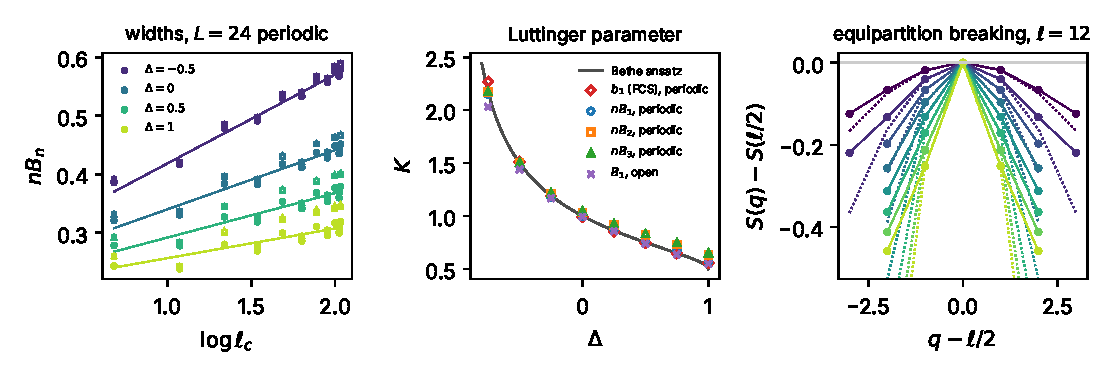
\includegraphics[width=\textwidth]{symmetry_resolved.pdf}
\caption{Periodic chain, $L=\SRL$. Left: $nB_n$ against $\log\ell_c$ for $n=1$ (filled circles), $2$ (squares) and $3$
(triangles); lines: slope $K/\pi^2$ (Bethe ansatz). Middle: $K$ from the fits of Table~\ref{tab:K}. Right:
$S(q)-S(\ell/2)$ at $\ell=\SRHalf$ for $\Delta\in\{\SRDeltas\}$ (dark to light); dotted: the Gaussian
form~\eqref{eq:gauss}, exact at $q-\ell/2=\pm1$.}\label{fig:sre}
\end{figure}

Tables~\ref{tab:K} and~\ref{tab:eq} and Figure~\ref{fig:sre} contain the results.

\paragraph{Number entanglement.} At these sizes most of the entanglement is number entanglement. $H(p)/S$ lies between
$\SRFracHMin$ and $\SRFracHMax$ and increases with $K$, and $H(p)$ equals the entropy $H_{\rm G}$ of the integer-sampled
Gaussian of width $B_1$ to within $\SRHSampledDevMax$ (Table~\ref{tab:eq}). The total entropy $S$ at $\ell=L/2$ varies
little with $\Delta$; the split~\eqref{eq:split} moves weight from $H(p)$ to the configurational part as $K$ decreases.

\paragraph{Widths and the $1/n$ law.} The widths $B_n$ of~\eqref{eq:Bdef} grow linearly in $\log\ell_c$
(Figure~\ref{fig:sre}, left). The $1/n$ law holds well for large $K$ and degrades as $K$ decreases. The spread of $nB_n$
over $n=1,2,3$ grows from $\SRSpreadMin\,\%$ of $B_1$ at $\Delta=-0.75$ to $\SRSpreadMax\,\%$ at $\Delta=1$
(Table~\ref{tab:eq}). The slopes of $2B_2$ and $3B_3$ give $K$ to within $0.1\,\%$ at $\Delta=-0.75$ ($2.172$ and $2.175$
against $2.173$), but exceed $K/\pi^2$ by $\SRKWidthHalfTwo\,\%$ and $\SRKWidthHalfThree\,\%$ at $\Delta=0.5$, and give
$\SRHeisKWidthThree$ for $n=3$ at $\Delta=1$ (Table~\ref{tab:K}). We attribute this to finite-size corrections, which our
fits do not model. In contrast, the variances $b_n$ for $n\ge2$ are dominated by the discreteness of $Q_A$; the widths
$B_n$ are the quantities in which the $1/n$ law is visible at $L\le\SRL$.

\paragraph{Breaking of equipartition.} Equipartition is clearly broken at $L=\SRL$.
$\delta S=S(q_0)-S(q_0\pm1)=G_1/(2B_1^2)$ ranges from $\SRdSMin$ to $\SRdSMax$ and increases as $K$ decreases
(Figure~\ref{fig:sre}, right). The Rényi-2 analogue $\delta S_2$ behaves in the same way. In agreement with the
mechanism of Section~\ref{sec:sre-model}, $G_1$ is nearly independent of $\ell$ while $B_1$ grows: over the even blocks
$4\le\ell\le L/2$ the slope of $G_1$ against $\log\ell_c$ is at most $\SRGSlopeRatioMax\,\%$ of that of $B_1$, and
$G_1$ changes by at most $\SRGRelChangeMax\,\%$ between $\ell=\SRQuarter$ and $\ell=\SRHalf$. The finite-size amplitude
$G_1(\Delta)$ at $\ell=\SRHalf$ increases from $0.0195$ at $\Delta=-0.75$ to $0.0518$ at $\Delta=0.75$, with $0.0512$ at
$\Delta=1$ (Table~\ref{tab:eq}). The quadratic dependence on $q$ is not yet reached: the ratio in Table~\ref{tab:eq} is
$\SRRatioMin$--$\SRRatioMax$ instead of $4$, and it decreases as $K$ decreases.

\paragraph{Luttinger parameter.} The full counting statistics $b_1$ give $K$ to within $\SRKFcsDevPct\,\%$ for
$\SRKFcsMidRange\le\Delta\le\SRKFcsMidRangeHi$. At $\Delta=-0.75$ the fit gives $2.267$ against $2.173$ (about $4\,\%$),
and at the isotropic point $\SRHeisKFcs$ instead of $0.5$. There the marginal operator causes logarithmic corrections, as
in the analysis of~\cite{song2012}, which we reproduce here by exact diagonalisation. The widths $B_1$ give $K$ to within
$\SRKWidthDevPct\,\%$ for $\Delta\le0.75$ in the periodic chain. The open chain, with a single entangling point,
deviates more at negative $\Delta$ (Table~\ref{tab:K}).

\subsection{Free fermions and comparison with Bonsignori, Ruggiero and Calabrese}\label{sec:sre-ff}

At $\Delta=0$ the chain is a free-fermion model, and the resolved quantities can be computed for much larger blocks from
the correlation matrix (Section~\ref{sec:validation}). Bonsignori, Ruggiero and Calabrese~\cite{bonsignori2019}
obtained the Fisher--Hartwig asymptotics of the charged moments. Their Gaussian (Eq.~(4.5) of~\cite{bonsignori2019}),
written in the variables of~\eqref{eq:gauss}, has $G_1\to1/(2\pi^2)$, and the breaking of equipartition at half filling
is~\cite[Eq.~(4.13)]{bonsignori2019}
\begin{equation}\label{eq:brc}
  S(q)-S(\langle Q_A\rangle)\simeq-\frac{\pi^2}4\,\frac{(q-\langle Q_A\rangle)^2}{(\log2\ell+1+\gamma_E)^2}.
\end{equation}
These are known results. We use them as a reference and measure the approach to them.
\begin{itemize}\itemsep0pt
\item \emph{Infinite XX chain.} For $\ell=\SRInfEll$, $b_1-(\log2\ell+1+\gamma_E)/\pi^2=\SRInfBDev$, and
$G_1^{(b)}=\partial_n(nb_n)|_{n=1}=\SRInfGOne$, while $1/(2\pi^2)=\SRInfGRef$. (Here $G_1^{(b)}$ is defined with the
variances $b_n$, which the script evaluates in closed form over the entanglement spectrum.) The exact $S(q_0)-S(q_0+1)$
is $\SRInfdSRatioFirst$ ($\ell=\SRInfdSEllFirst$) and $\SRInfdSRatio$ ($\ell=\SRInfdSEll$) times the value
of~\eqref{eq:brc}, and the ratio of Table~\ref{tab:eq} is $\SRInfRatio$ at $\ell=\SRInfdSEll$.
\item \emph{Periodic XX ring, $\ell=L/2$.} The ratio is $\SRRingRatioFirst$ at $L=\SRRingLfirst$ (our value in
Table~\ref{tab:eq}) and $\SRRingRatio$ at $L=\SRRingLmax$, and $G_1=\SRRingGOne$ at $L=\SRRingLmax$, against $\SRXXGOne$ at
$L=\SRL$.
\end{itemize}
The asymptotic amplitude is therefore approached slowly, with deviations of several per cent even at $\ell$ in the
thousands. This puts the values at $L=\SRL$ in perspective. For $\Delta\ne0$ the $G_1$ of Table~\ref{tab:eq} are
finite-size values of the non-universal amplitudes discussed in~\cite{estienne2021}; we have not compared them with the
twisted overlaps computed there.

\paragraph{What is reproduced and what is new.} Equipartition, the $(K/\pi^2)\log\ell$ charge variance with its
oscillating correction, and the $\log^{-2}\ell$ breaking are
known~\cite{goldstein2018,xavier2018,bonsignori2019,song2012,estienne2021}. For free fermions the amplitude of the
breaking is known exactly~\cite{bonsignori2019}, and~\eqref{eq:id} is Eq.~(2.6) of~\cite{bonsignori2019} written with
$p_n$. Larger sizes have been reached by DMRG and quantum Monte Carlo~\cite{laflorencie2014,xavier2018,chen2026}. Our
additions are modest. They are the integer-sampled widths $B_n$, for which the $1/n$ law is visible at $L\le\SRL$ (well
for large $K$, less so near $\Delta=1$); the finite-size amplitudes $G_1(\Delta)$ for $\Delta\ne0$; the Luttinger
parameter from the charge statistics, to within $\SRKFcsDevPct\,\%$ for $\SRKFcsMidRange\le\Delta\le\SRKFcsMidRangeHi$;
and an exact check of the free-fermion amplitude, including how slowly it is approached.

\section{Validation}\label{sec:validation}

All computations are in double precision. The scripts \code{scripts/permutational.py} and
\code{scripts/symmetry_resolved.py} of the repository~\cite{lib} compute the checks below together with the results,
and the unit tests in \code{tests/test_permutational.py} and \code{tests/test_symmetry_resolved.py} repeat them at
small sizes with fixed tolerances. Deviations are maximal absolute deviations unless stated otherwise.

\subsection{Part A}

The checks were run in the script's check mode (\PMDevice).
\begin{enumerate}\itemsep1pt
\item[(A1)] \emph{Exact generator.} The banded generator, with all nine terms of~\eqref{eq:general} switched on, is
compared with the exact Lindblad generator on $(\C^2)^{\otimes N}$, compressed to $\M$ through Dicke bases built
independently from $J^2$ and $J_z$ (eigenvectors of $J^2$ at $m=j$, then lowering with $J_-$). For random
permutation-invariant states it agrees to $\PMFullErr$ for $N\le\PMFullNmax$, and the exact generator maps $\M$ into
itself up to round-off. An RK4 trajectory computed on $(\C^2)^{\otimes\PMTrajN}$ gives the same blocks to
$\PMTrajErr$.
\item[(A2)] \emph{Generic route.} \code{dynamics.lindblad_evolve} with the local jumps as \code{InterSectorChannel}
(RK4) agrees with the banded generator to $\PMLibErr$ ($N=\PMLibN$; $\PMLibSecGeneric$~s against $\PMLibSecBanded$~s).
The second-order Kraus integrator of the same function agrees to $\PMLibKrausErr$.
\item[(A3)] \emph{PIQS.} Against \texttt{qutip.piqs}~\cite{shammah2018} (QuTiP~\PMPiqsVersion~\cite{lambert2026}), whose
local dephasing rate is $4\gamma_\phi$ in our convention, the generators agree to a relative $\PMPiqsGenErr$, limited by
the single-precision rates of PIQS. Trajectories of~\eqref{eq:btc} ($\gamma=0.1\kappa$, $\gamma_\phi=0.025\kappa$,
$\kappa t\le10$) agree for $N=\PMPiqsNs$ to $\PMPiqsTrajErr$ in $m_z$ and to $\PMPiqsBlockErr$ in the final blocks.
The steady states (null vectors of the two generators) agree for $N=\PMPiqsSsNs$ to $\PMPiqsSsErr$. For $N=\PMPiqsNmax$
one trajectory took $\PMPiqsSecOurs$~s here and $\PMPiqsSecBuild+\PMPiqsSecSolve$~s with PIQS (Liouvillian,
\texttt{mesolve}).
\item[(A4)] \emph{Superradiance.} Pure collective decay $\D[J_-]$ (rate $\Gamma=1$) from $|S,S\rangle$ is a pure death
process with rates $\Gamma(S+m)(S-m+1)$, so $\int_0^\infty P(m>0)\,dt=\sum_{m=1}^S[\Gamma(S+m)(S-m+1)]^{-1}=
H_N/(\Gamma(N+1))$, with the harmonic number $H_N$. Table~\ref{tab:sr} reproduces this to $\PMSRErr$ for
$N\le\PMSRNmax$. It also shows the superradiant delay $t_D\approx\ln N/(\Gamma N)$ and the reduction of the peak of
the mean intensity below the mean-field value $\Gamma N^2/4$ by the fluctuations of the delay~\cite{dicke1954,gross1982}.
\item[(A5)] \emph{Product states.} Local emission, pumping and dephasing alone keep a product state a product of
identical qubit states. Then $\langle J_z\rangle$, $\langle J_x\rangle$ and $\langle J^2\rangle$ follow from the Bloch
equations of one qubit, and the spin distribution is $p_j=m_j\sum_{m=-j}^j\lambda_+^{S+m}\lambda_-^{S-m}$ with the
eigenvalues $\lambda_\pm$ of the one-qubit state. For $N=\PMProdN$ ($\gamma_-,\gamma_+,\gamma_z=0.3,0.1,0.2$, initial polar
angle $2\pi/3$, $t\le2$) the moments agree to a relative $\PMProdErr$ and $\sum_j|p_j-p_j^{\rm exact}|=\PMProdPjErr$. This tests the
multiplicities in~\eqref{eq:kraus} far beyond the reach of the full space.
\item[(A6)] \emph{Time step.} Halving the RK4 step changes $m_z$ by at most $\PMConvMz$ and $\tau$ by at most
$\PMConvTau$ ($N=\PMConvN$, all ten parameter sets, $\kappa t\le30$).
\item[(A7)] \emph{Unit tests} (tolerance $10^{-12}$ unless stated). The algebra has $\sum_j(2j+1)m_j=2^N$; the collective
operators are the restrictions of those on $(\C^2)^{\otimes N}$; $\Phi^*(1)$ equals $N/2+J_z$, $N/2-J_z$, $N$ (also with
truncation); the banded generator equals the exact one for $N=2,\dots,6$; \code{local_jump} equals
$\sum_iL_i\rho L_i^*$ compressed to $\M$ ($N=5$); the generic and banded routes agree for a batch of two parameter sets;
a full-space RK4 trajectory agrees to $10^{-13}$ ($N=4$); the real algebra with drive about $y$ reproduces the complex
computation ($10^{-13}$, $N=9$); the product-state formulas hold for $N=30$ ($10^{-10}$ for the moments, $10^{-8}$
for $\langle J^2\rangle$ and $p_j$); the death-process integral holds to a relative $10^{-6}$ ($N=12$); the truncated
blocks satisfy $0\le\sigma^{\rm trunc}_j\le\sigma_j$ and the error bound of Section~\ref{sec:schurweyl} ($N=10$,
$j_{\min}=3$); generator and steady state agree with PIQS ($N=6$, relative $10^{-5}$); and the lifetime routine returns
$\tau=5+\pi/4$ to within $0.06$ for $m_z=-e^{-t/5}\cos2t$, and $\tau=\infty$ for the mean-field solution without local
terms.
\end{enumerate}

\begin{table}[t]
\centering\small
\caption{Check (A4), pure collective decay from $|S,S\rangle$ ($\Gamma=1$): the integral of $P(m>0)$ against the exact
value $H_N/(N+1)$, the time $t_D$ of the peak of the mean intensity $\Gamma\langle J_+J_-\rangle$ in units of $\ln N/N$,
and the peak in units of $N^2/4$ (mean field: $1$ and $1$ for $N\to\infty$).}\label{tab:sr}
\begin{tabular}{rccccc}
\toprule
$N$ & $\int P(m>0)\,dt$ & $H_N/(N+1)$ & rel.\ dev. & $t_DN/\ln N$ & $I_{\max}/(N^2/4)$\\
\midrule
\PMSRRows
\bottomrule
\end{tabular}
\end{table}

\subsection{Part B}

The checks were run together with the results (\SRMode\ mode, \SRDevice).
\begin{enumerate}\itemsep1pt
\item[(B1)] \emph{Free fermions.} For $\Delta=0$ the Jordan--Wigner transformation gives free fermions, the periodic bond
carrying the sign $(-1)^{N-1}$. With the eigenvalues $\nu_j$ of the correlation matrix restricted to
$A$~\cite{peschel2003}, flux insertion~\cite{goldstein2018} gives $Z_n(\alpha)=\prod_j[\nu_j^ne^{i\alpha}+(1-\nu_j)^n]$.
This is a polynomial of degree $\ell$ in $e^{i\alpha}$, so a discrete Fourier transform on $\ell+1$ points gives $Z_n(q)$
exactly, and $\Tr\Pi_q\rho_A\log\rho_A$ is the transform of $\partial_nZ_n(\alpha)|_{n=1}$. For every block, $p(q)$,
$\Tr\Pi_q\rho_A\log\rho_A$, $Z_{2,3}(q)$, $b_{1,2}$, $B_1$ and $G_1$ agree with the library to $\SRFFDenseDev$ (dense
sector, $L=\SRFFLDense$) and $\SRFFLanczosDev$ (Lanczos, $L=\SRL$), periodic and open. $S(q)$, $S_2(q)$, $S_3(q)$ agree
to $\SRFFLanczosDevS$ where $p(q),p_n(q)>\SRPCmp$ (the transform has absolute round-off). The ground energies agree with the
free-fermion values to $\SRFFEDev$.
\item[(B2)] \emph{Full Hilbert space.} The dense ground state in the $2^L$-dimensional space (NumPy, no symmetry used,
$L=\SRFullL$, $\Delta\in\{\SRFullDeltas\}$, periodic and open) and the projections $\Pi_q\rho_A\Pi_q$ of the
$2^\ell\times2^\ell$ matrix $\rho_A$ give $p(q)$ and $S(q)$ for all $\ell<L$ to $\SRFullDev$. The part of $\rho_A$ between
different charges is below $\SRFullOff$.
\item[(B3)] \emph{Three routes to $\rho_A$.} The pair blocks~\eqref{eq:rhoA}, \code{SpinChain.reduced_state} of
$|\psi\rangle\langle\psi|$ and \code{composite.partial_trace} in the fused product give the same $\rho_A$ to
$\SRRoutesDev$.
\item[(B4)] \emph{QuSpin.} QuSpin~\cite{weinberg2017} (reduced density matrix projected on the charges) agrees for
$L=\SRQuSpinL$, $\Delta=\SRQuSpinDelta$, periodic and open, to $\SRQuSpinDev$ in $p(q)$ and $S(q)$, and to $\SRQuSpinE$ in
the ground energy.
\item[(B5)] \emph{Unit tests.} The Bethe-ansatz $K$ takes the values $\frac32,1,\frac34,\frac12$ at
$\Delta=-\frac12,0,\frac12,1$. The batched Hamiltonian equals the library's sector Hamiltonian for each $\Delta$. The
free-fermion comparison (B1) holds at $L=12$ (tolerances $10^{-13}$ for $p$, $Z_n$; $10^{-8}$ for $S(q)$, $S_n(q)$).
The full-space comparison (B2) holds at $L=8$ for $\Delta\in\{-0.6,0,0.3,1\}$, and the three routes (B3) agree to
$10^{-14}$ at $L=10$. The split~\eqref{eq:split} holds to $10^{-13}$, the first identity~\eqref{eq:id} to $10^{-12}$ and
the second, with a central difference in $n$, to $10^{-8}$. $G_1=\partial_n(nB_n)|_{n=1}$ holds to $10^{-7}$, and the
Gaussian form~\eqref{eq:gauss} is exact at $q_0\pm1$ to $10^{-12}$. For the infinite XX chain at $\ell=400$,
$|b_1-(\log2\ell+1+\gamma_E)/\pi^2|<10^{-6}$, $|G_1^{(b)}-1/(2\pi^2)|<2\times10^{-5}$, and $S(q_0)-S(q_0+1)$ lies
between $0.9$ and $1$ times the value of~\eqref{eq:brc}; these last three are observations, not proofs.
\end{enumerate}

\section{Outlook}\label{sec:outlook}

In both problems the symmetry structure turns an intractable dimension into a manageable one, $\PMDimNmax$ entries
instead of $\PMDimFullNmax$ for $N=\PMNmax$ spins, and a sector of dimension $\SRDim$ with blocks of $\rho_A$ of size
at most $\binom{12}{6}=924$ for $L=\SRL$. The decisive ingredients were the representation of permutation-invariant
local dissipators as completely positive maps between sectors, and the sector form of a bipartite pure state.

All numbers reported here come from CPU runs: Part~A in the check mode of the script ($N\le\PMNmax$, one thread) and
Part~B in its full mode (two threads). The banded generator costs $O(N^3)$ per step with a number of steps that grows
as $N$. The script has a mode with $N$ up to $200$ and longer runs designed for a GPU; GPU runs will extend $N$, and the
batched Lanczos runs to larger $L$. Such runs would show whether the deviations from the additive
rule~\eqref{eq:rule} keep decreasing for the larger rates and keep drifting for the smallest ones. For the XXZ chain they
would tell how the spread of $nB_n$ and the amplitudes $G_1(\Delta)$ evolve with $L$. Other directions are local
pumping and collective dephasing, which the generator~\eqref{eq:general} already contains; other definitions of the
lifetime; a comparison of $G_1(\Delta)$ with the twisted overlaps of~\cite{estienne2021}; and other conserved charges,
for which only the sector structure of~\eqref{eq:rhoA} changes.

\paragraph{Code and data availability.} The library, the scripts that compute all numbers, tables and figures, the
generated data (\code{man/article/generated/permutational.json} and \code{symmetry_resolved.json}) and the tests
are available at \url{https://github.com/andre-a-no/von_neumann_type_i} (MIT licence)~\cite{lib}.

{\sloppy
\begin{thebibliography}{99}
\bibitem{baragiola2010} B.~Q.~Baragiola, B.~A.~Chase, J.~Geremia, ``Collective uncertainty in partially polarized
  and partially decohered spin-1/2 systems'', Phys.\ Rev.\ A 81 (2010), 032104.
\bibitem{bartlett2007} S.~D.~Bartlett, T.~Rudolph, R.~W.~Spekkens, ``Reference frames, superselection rules, and
  quantum information'', Rev.\ Mod.\ Phys.\ 79 (2007), 555--609.
\bibitem{bonsignori2019} R.~Bonsignori, P.~Ruggiero, P.~Calabrese, ``Symmetry resolved entanglement in free fermionic
  systems'', J.\ Phys.\ A 52 (2019), 475302.
\bibitem{carollo2021} F.~Carollo, I.~Lesanovsky, ``Exactness of mean-field equations for open Dicke models with an
  application to pattern retrieval dynamics'', Phys.\ Rev.\ Lett.\ 126 (2021), 230601.
\bibitem{chase2008} B.~A.~Chase, J.~M.~Geremia, ``Collective processes of an ensemble of spin-1/2 particles'',
  Phys.\ Rev.\ A 78 (2008), 052101.
\bibitem{chen2026} K.~Chen, W.~Jia, X.~Li, R.~Meyer, J.~Zhao, ``Detecting symmetry-resolved entanglement: a quantum
  Monte Carlo approach'', arXiv:2604.02307 (2026).
\bibitem{dicke1954} R.~H.~Dicke, ``Coherence in spontaneous radiation processes'', Phys.\ Rev.\ 93 (1954), 99--110.
\bibitem{estienne2021} B.~Estienne, Y.~Ikhlef, A.~Morin-Duchesne, ``Finite-size corrections in critical
  symmetry-resolved entanglement'', SciPost Phys.\ 10 (2021), 054.
\bibitem{fulton1991} W.~Fulton, J.~Harris, \emph{Representation Theory: A First Course}, Graduate Texts in
  Mathematics 129, Springer, 1991.
\bibitem{gegg2017} M.~Gegg, M.~Richter, ``PsiQuaSP -- a library for efficient computation of symmetric open
  quantum systems'', Sci.\ Rep.\ 7 (2017), 16304.
\bibitem{goldstein2018} M.~Goldstein, E.~Sela, ``Symmetry-resolved entanglement in many-body systems'',
  Phys.\ Rev.\ Lett.\ 120 (2018), 200602.
\bibitem{gross1982} M.~Gross, S.~Haroche, ``Superradiance: an essay on the theory of collective spontaneous
  emission'', Phys.\ Rep.\ 93 (1982), 301--396.
\bibitem{iemini2018} F.~Iemini, A.~Russomanno, J.~Keeling, M.~Schir\`o, M.~Dalmonte, R.~Fazio, ``Boundary time
  crystals'', Phys.\ Rev.\ Lett.\ 121 (2018), 035301.
\bibitem{kiefer2020} M.~Kiefer-Emmanouilidis, R.~Unanyan, M.~Fleischhauer, J.~Sirker, ``Evidence for unbounded growth
  of the number entropy in many-body localized phases'', Phys.\ Rev.\ Lett.\ 124 (2020), 243601.
\bibitem{kirton2017} P.~Kirton, J.~Keeling, ``Suppressing and restoring the Dicke superradiance transition by
  dephasing and decay'', Phys.\ Rev.\ Lett.\ 118 (2017), 123602.
\bibitem{laflorencie2014} N.~Laflorencie, S.~Rachel, ``Spin-resolved entanglement spectroscopy of critical spin
  chains and Luttinger liquids'', J.\ Stat.\ Mech.\ (2014), P11013.
\bibitem{lambert2026} N.~Lambert et al., ``QuTiP~5: The Quantum Toolbox in Python'', Phys.\ Rep.\ 1153 (2026),
  1--62; arXiv:2412.04705.
\bibitem{lib} I.~Nikolaeva, A.~Novikov, ``Finite-dimensional Type I von Neumann algebras in PyTorch: a
  GPU-accelerated framework for random block-diagonal operators'', arXiv:2606.15882 (2026);
  code: \url{https://github.com/andre-a-no/von_neumann_type_i}.
\bibitem{liu2026} Z.~Liu, Y.~Li, Z.~Fei, X.~Wang, ``Boundary time crystals beyond mean-field theory: a stroboscopic
  rotating-wave approximation'', Phys.\ Rev.\ A 114 (2026), 012211; arXiv:2510.03028.
\bibitem{lukin2019} A.~Lukin, M.~Rispoli, R.~Schittko, M.~E.~Tai, A.~M.~Kaufman, S.~Choi, V.~Khemani, J.~L\'eonard,
  M.~Greiner, ``Probing entanglement in a many-body-localized system'', Science 364 (2019), 256--260.
\bibitem{nemeth2025} D.~Nemeth, A.~Principi, A.~Nazir, ``Analytical solution of boundary time crystals via the
  superspin basis'', arXiv:2507.06998 (2025).
\bibitem{paszke2019} A.~Paszke et al., ``PyTorch: An imperative style, high-performance deep learning
  library'', NeurIPS 2019.
\bibitem{peschel2003} I.~Peschel, ``Calculation of reduced density matrices from correlation functions'',
  J.\ Phys.\ A 36 (2003), L205--L208.
\bibitem{piccitto2021} G.~Piccitto, M.~Wauters, F.~Nori, N.~Shammah, ``Symmetries and conserved quantities of
  boundary time crystals in generalized spin models'', Phys.\ Rev.\ B 104 (2021), 014307.
\bibitem{prazeres2021} L.~F.~dos~Prazeres, L.~da~Silva~Souza, F.~Iemini, ``Boundary time crystals in collective
  $d$-level systems'', Phys.\ Rev.\ B 103 (2021), 184308.
\bibitem{shammah2018} N.~Shammah, S.~Ahmed, N.~Lambert, S.~De~Liberato, F.~Nori, ``Open quantum systems with local
  and collective incoherent processes: Efficient numerical simulations using permutational invariance'',
  Phys.\ Rev.\ A 98 (2018), 063815.
\bibitem{song2012} H.~F.~Song, S.~Rachel, C.~Flindt, I.~Klich, N.~Laflorencie, K.~Le~Hur, ``Bipartite fluctuations as
  a probe of many-body entanglement'', Phys.\ Rev.\ B 85 (2012), 035409.
\bibitem{takesaki2002} M.~Takesaki, \emph{Theory of Operator Algebras I}, Springer, 2002.
\bibitem{tucker2018} K.~Tucker, B.~Zhu, R.~J.~Lewis-Swan, J.~Marino, F.~Jimenez, J.~G.~Restrepo, A.~M.~Rey,
  ``Shattered time: can a dissipative time crystal survive many-body correlations?'', New J.\ Phys.\ 20 (2018),
  123003.
\bibitem{weinberg2017} P.~Weinberg, M.~Bukov, ``QuSpin: a Python package for dynamics and exact diagonalisation of
  quantum many body systems part I: spin chains'', SciPost Phys.\ 2 (2017), 003.
\bibitem{xavier2018} J.~C.~Xavier, F.~C.~Alcaraz, G.~Sierra, ``Equipartition of the entanglement entropy'',
  Phys.\ Rev.\ B 98 (2018), 041106.
\end{thebibliography}
}

\end{document}
